\section{Introduction}

Astrophysical and cosmological observations provide strong evidence that about 27\% of the energy density of the universe is made out of Dark Matter (DM). 
The DM hypothesis is based on the existence of a non-luminous, non-baryonic, and non-relativistic particle, the nature of which 
is yet unknown~\cite{Harvey1462,WMAP:9years,PLANCK}. 
Many well-motivated theoretical extensions of the Standard Model of particle physics predict the existence of one or more particles with the required properties, with masses and cross sections typically of the order of the weak scale. Such particles are collectively known as Weakly Interacting Massive Particles (WIMPs)~\cite{Bertone:2010zza}. The hypothesis that dark matter is constituted primarily of WIMPs is currently being tested by many experiments, either indirectly by seaching for evidence of their possible decay or annihilation in astrophysical processes, by searching for evidence of their direct production at collider experiments, or by directly measuring the rare scattering of astrophysical WIMPs from target nuclei in Earth-based laboratories~\cite{xe100_run_combination,PANDAX,LUXnew,COGENT,CDMSlite,CREST,DAMA}. We report on a search of this latter kind.


The traditional approach for computing predictions of the rate of WIMP-nucleon scattering has been to take only leading-order terms in a WIMP-nucleon effective field theory (EFT) with a very simple treatment of nuclear structure~\cite{LEWIN}. This leads to two main types of interactions, which are commonly labelled ``Spin Independent'' (SI) and ``Spin Dependent'' (SD). However, in recent years many authors have pointed out that in certain theories these interactions may be suppressed or nonexistent, such that otherwise subleading interactions may dominate the scattering process~\cite{Chang:2009yt}. To account for this possibility in a systematic way, a more sophisticated EFT approach has been developed ~\cite{Fitzpatrick:2012ib,Anand:MathTools,Fitzpatrick:MathTools}. In this new approach an effective Lagrangian describing the WIMP-nucleus interaction is constructed, 
%that 
\ale{this} takes into account all Galilean-invariant operators up to second order in the momentum exchange. In this framework, new operators associated with different types of nuclear responses are introduced along with the standard SI and SD ones, resulting in a set of fourteen operators $\mathcal{O}_i$ which may couple independently to protons and neutrons. In Eqs. (\ref{eq:OpDef}) we list these operators following the convention from~\cite{Anand:MathTools}. The operators depend explicitly on 4 linearly independent quantities: $\vec{v}^{\perp} \equiv \vec{v} + \frac{\vec{q}}{2\mu_N} $, the relative perpendicular velocity between the WIMP and the nucleon, $\vec{q}$, the momentum transferred in the scattering event, and $\vec{S}_\chi$, $\vec{S}_N$, the WIMP and nucleon spins. $\mathcal{O}_2$ is not considered here as it cannot be obtained from a relativistic operator at leading order.
%

\begingroup
\belowdisplayskip=0pt
\begin{align*}
\begin{split} 
&\mathcal{O}_1 = 1_{\chi} 1_N  \\
%&\mathcal{O}_2 = (v^{\perp})^2 \\
&\mathcal{O}_3 = i\vec{S}_N\cdot (\frac{\vec{q}}{m_N}\times\vec{v}^\perp) \\
&\mathcal{O}_4 = \vec{S}_{\chi}\cdot \vec{S}_N \\
&\mathcal{O}_5 = i\vec{S}_{\chi}\cdot (\frac{\vec{q}}{m_N}\times\vec{v}^\perp) \\
&\mathcal{O}_6 = (\vec{S}_{\chi} \cdot \frac{\vec{q}}{m_N})(\vec{S}_N \cdot \frac{\vec{q}}{m_N}) \\
&\mathcal{O}_7 = \vec{S}_N \cdot \vec{v}^\perp \\
&\mathcal{O}_8 = \vec{S}_{\chi} \cdot \vec{v}^\perp  \\
\end{split}
\begin{split}
&\mathcal{O}_9 = i\vec{S}_{\chi} \cdot(\vec{S}_N \times \frac{\vec{q}}{m_N}) \\
&\mathcal{O}_{10} = i\vec{S}_N \cdot (\frac{\vec{q}}{m_N}) \\
&\mathcal{O}_{11} = i\vec{S}_{\chi} \cdot (\frac{\vec{q}}{m_N}) \\
&\mathcal{O}_{12} = \vec{S}_\chi \cdot (\vec{S}_N \times \vec{v}^\perp) \\
&\mathcal{O}_{13} = i(\vec{S}\chi \cdot \vec{v}^\perp)(\vec{S}_N \cdot \frac{\vec{q}}{m_N})\\
&\mathcal{O}_{14} = i(\vec{S}_\chi \cdot \frac{\vec{q}}{m_N})(\vec{S}_N \cdot \vec{v}^\perp) \\
\end{split}
\end{align*}
\endgroup
\begingroup
\abovedisplayskip=0pt
\begin{align}
&\mathcal{O}_{15} = -(\vec{S}_\chi \cdot \frac{\vec{q}}{m_N})\left[(\vec{S}_N \times \vec{v}^\perp)\cdot \frac{\vec{q}}{m_N}\right]
\label{eq:OpDef}
\end{align}
\endgroup

Unlike the more commonly studied types of interaction (SI,SD), which are not suppressed when $\vec{q} \rightarrow 0$ and for which the scattering rate on nucleons is expected to be largest for low energy nuclear recoils, some of the new EFT operators depend explicitly on $\vec{q}$ and so their interaction cross section is suppressed for low momentum transfers. Consequently, their scattering rate peaks at non-zero nuclear recoil energy. For sufficiently high WIMP masses, this may even occur outside typical analysis windows, usually below $ 43\,\keVr$ (nuclear recoil equivalent
energy), designed to search for SI and SD interactions (see Figure~\ref{fig:dRdE}). Due to the theoretical bias of only considering SI and SD interactions, high energy nuclear recoils remain unexplored in many experiments.
	    
%	    Another assumption that can be relaxed is that WIMP should scatter elastically, however there are models in which the incoming and outgoing WIMPs have different mass states ~\cite{InelasticIntro}. In the case where the outgoing state is more massive than the incoming state the event rate at low recoil energies can again be suppressed, hence analyses which apply an upper energy bound lose sensitivity to these types of interactions. Recently an inelastic adaptation of the EFT operator framework discussed above was developed~\cite{InelasticMath}. The operators presented in~\ref{eq:OpDef} are modified such that $\vec{v}^\perp_{inelastic} = \vec{v}^\perp_{elastic} +\frac{\delta}{\vert{\vec{q}}\vert^2}\vec{q}$. \RanComment{We should add here the dependency of $v_{min}$ on $\delta$}      
	    Another typical assumption that can be relaxed is that WIMPs should scatter elastically with nuclei. There exist dark matter models in which the incoming and outgoing WIMPs have different mass states ~\cite{InelasticIntro} separated by a keV-scale splitting. In the case where the outgoing state is more massive than the incoming state, the cross section for low recoil energies can again be suppressed, this time by scattering kinematics. Recently an inelastic adaptation of the EFT operator framework discussed above was developed~\cite{InelasticMath}. In this case the operators presented in Eqs.~\ref{eq:OpDef} are modified such that $\vec{v}^\perp_{inelastic} = \vec{v}^\perp_{elastic} +\frac{\delta_m}{\vert{\vec{q}}\vert^2}\vec{q}$. We consider this case in section \ref{subsubsec:Inelastic}.
	    
The EFT framework of \cite{Fitzpatrick:2012ib} is constructed at the WIMP-nucleon level and so each operator may be present independently for protons and neutrons, though UV models can of course correlate their couplings. The full EFT thus has 28 coupling parameters in addition to the WIMP mass (plus a mass splitting~$\delta$ in the inelastic case). This parameter space is too large to explore in full, so we take a similar approach to the SI/SD case 
and assume only one active operator at a time, considering it equally coupled to protons and neutrons (the ``isoscalar'' case). However, to facilitate the full exploitation of these results by the community, we provide in supplementary material a set of tools for converting any theoretical recoil spectrum $\mathrm{d}R/\mathrm{d}E$ into an accurate event rate prediction for this analysis, including all detector response and analysis efficiency effects. This may help to set a mildly conservative but quite accurate limit on arbitrary models in the full EFT parameter space, or any other particle dark matter model for which one can supply the expected recoil spectrum.

Motivated by these EFT extensions of the standard WIMP framework, we report on an analysis extending the searched recoil energy range up to $240~\keVr$ for the first time in the \Xehund\ experiment, and present exclusion limits on all operators for both the elastic and the inelastic WIMP cases.     


\begin{figure}[t!]
\centerline{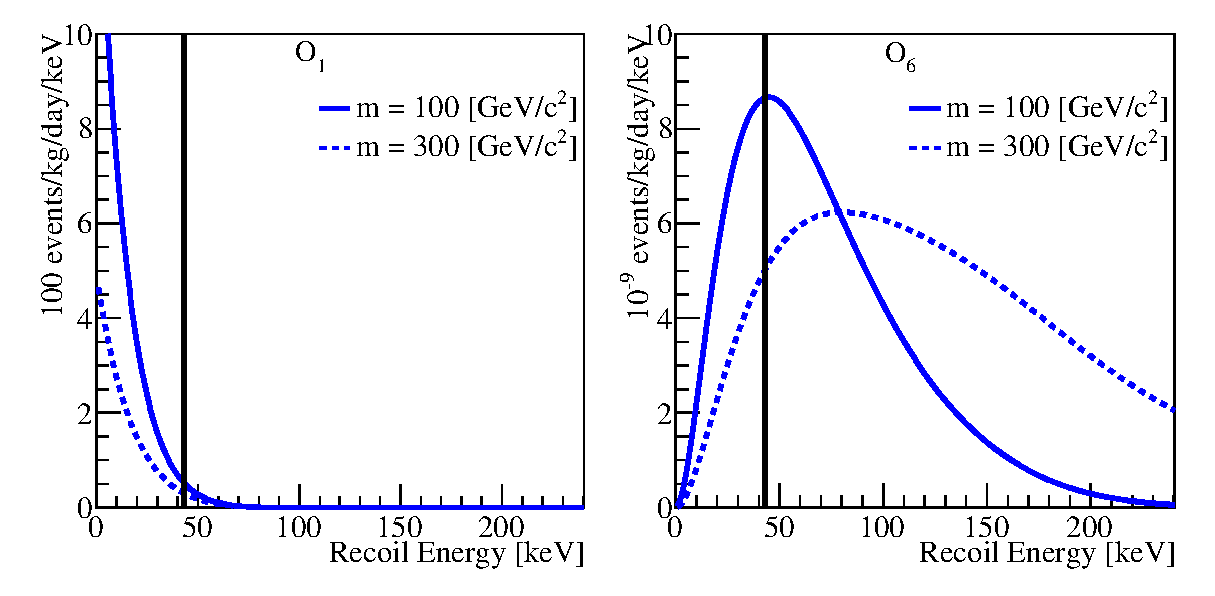
\includegraphics[width=1.\linewidth]{Figures/drdeO1O6.eps}}
\caption{Example EFT recoil spectra for elastic scattering of spin-$1/2$ WIMPs on Xenon nuclei (weighted according to the isotope abundances in the XENON100 experiment). Left(right) shows the predicted spectra for EFT operator $\mathcal{O}_1$($\mathcal{O}_6$). The normalization is controlled by the coupling coefficient of each EFT operator and the experimental exposure. The solid vertical line at $43~\keVr$ shows the approximate division between the two signal regions used in this analysis. As shown, the standard SI ($\mathcal{O}_1$) spectrum is concentrated mainly in the already-explored energy region. However, some EFT operators, for certain WIMP masses, predict a significant fraction of recoil events above the upper energy cut used in the standard spin-independent analysis, motivating an extension of this cut. The highest recoil energy shown in the plots, $240~\keVr$, roughly corresponds the highest energy accounted for this analysis.}
\label{fig:dRdE}
\end{figure}

\section{The \Xehund\  Detector}
The \Xehund\ detector is a cylindrical %30\,cm~height, 30\,cm~diameter, 
dual-phase xenon (liquid and gas) time projection chamber (TPC). It is installed at the Laboratori Nazionali del Gran Sasso (LNGS) in Italy
and contains 161\,kg of liquid xenon (LXe), of which 62\,kg function as the active target ~\cite{xe100_instr2012}. 
The detector uses of a total of 178~1-inch square Hamamatsu R8520-AL photomultiplier tubes (PMTs) employed in two arrays, one in the gas phase at the top of the TPC, and the other at the bottom, immersed in the LXe. 

A particle interacting with the LXe deposits energy that creates both
prompt scintillation ($S1$) and delayed proportional scintillation ($S2$) which are detected using the two PMT arrays. The $S2$ signal is produced by ionization electrons, drifted in an electric field of $530$V/cm towards the liquid-gas interface, where they are extracted to the gas phase using a stronger electric field of $\sim12$kV/cm in which the proportional scintillation occurs. 
The spatial distribution of the $S2$ signal on the top PMT array, together with the time difference between $S1$ and $S2$ signals, provide respectively X-Y and Z position information for each interaction, allowing 3D position reconstruction to be achieved.
%determines the X-Y position, while the time difference between the two signals gives the z-coordinate, and thus a 3D position reconstructions is achieved.

Interaction in different locations of  the detector have different signatures. In order to take these effects into account, a correction is applied based on light and charge collection efficiency maps. These maps are prepared using calibration sources ranging up to energies well above 240$\keVr$, which is the highest energy recoil considered in this paper. The corrected signals ($cS1$,$cS2$) are spatially independent and uniform to all interactions~\cite{xe100_instr2012}. Note that some of the top PMTs saturate for large S2 signals and we therefore use in this analysis only the bottom PMT array to infer the energy scale in $S2$.

The $S2/S1$ ratio is known to differ between nuclear recoil (NR) and electronic recoil (ER) interactions, and is thus used as a discriminating variable between a WIMP signal and ER background. The logarithm of this ratio, log($cS2_b/cS1$) is referred later in the text as the discriminating "$y$" variable.

% between ER background coming from $\gamma$, $\beta$ and NR signal coming from a WIMP. 

